
\documentclass[a4paper,UKenglish,cleveref, autoref, thm-restate]{lipics-v2021}
%This is a template for producing LIPIcs articles.
%See lipics-v2021-authors-guidelines.pdf for further information.
%for A4 paper format use option "a4paper", for US-letter use option "letterpaper"
%for british hyphenation rules use option "UKenglish", for american hyphenation rules use option "USenglish"
%for section-numbered lemmas etc., use "numberwithinsect"
%for enabling cleveref support, use "cleveref"
%for enabling autoref support, use "autoref"
%for anonymousing the authors (e.g. for double-blind review), add "anonymous"
%for enabling thm-restate support, use "thm-restate"
%for enabling a two-column layout for the author/affilation part (only applicable for > 6 authors), use "authorcolumns"
%for producing a PDF according the PDF/A standard, add "pdfa"

%\pdfoutput=1 %uncomment to ensure pdflatex processing (mandatatory e.g. to submit to arXiv)
%\hideLIPIcs  %uncomment to remove references to LIPIcs series (logo, DOI, ...), e.g. when preparing a pre-final version to be uploaded to arXiv or another public repository

\usepackage{wrapfig}
\usepackage{tikz-qtree}
\usetikzlibrary{positioning}
\usetikzlibrary{arrows.meta}
\usetikzlibrary{arrows,shapes,quotes}

\usepackage{todonotes}

%\graphicspath{{./graphics/}}%helpful if your graphic files are in another directory

\bibliographystyle{plainurl}% the mandatory bibstyle

\title{Embedding Intuitionistic into Classical Logic} %TODO Please add

%\titlerunning{Dummy short title} %TODO optional, please use if title is longer than one line

\author{Alexander {Pluska}}{Faculty of Mathematics, Universtät Wien, Austria}{e11941874@student.tuwien.ac.at}{https://orcid.org/my-orcid?orcid=0000-0002-7709-3335}{}%TODO mandatory, please use full name; only 1 author per \author macro; first two parameters are mandatory, other parameters can be empty. Please provide at least the name of the affiliation and the country. The full address is optional. Use additional curly braces to indicate the correct name splitting when the last name consists of multiple name parts.

\author{Florian Zuleger}{Institute of Logic and Computation, Technische Universität Wien, Austria}{florian.zuleger@tuwien.ac.at}{https://orcid.org/0000-0003-1468-8398}{}

\authorrunning{A. Pluska and F. Zuleger} %TODO mandatory. First: Use abbreviated first/middle names. Second (only in severe cases): Use first author plus 'et al.'

\Copyright{Alexander Pluska and Florian Zuleger} %TODO mandatory, please use full first names. LIPIcs license is "CC-BY";  http://creativecommons.org/licenses/by/3.0/

\ccsdesc[100]{\textcolor{red}{Theory of Computation Logic Constructive Mathematics}} %TODO mandatory: Please choose ACM 2012 classifications from https://dl.acm.org/ccs/ccs_flat.cfm

\keywords{Intuitionistic Logic, Automated Reasoning, Propositional Logic, First-order Logic, QBF} %TODO mandatory; please add comma-separated list of keywords

\category{} %optional, e.g. invited paper

\relatedversion{} %optional, e.g. full version hosted on arXiv, HAL, or other respository/website
%\relatedversiondetails[linktext={opt. text shown instead of the URL}, cite=DBLP:books/mk/GrayR93]{Classification (e.g. Full Version, Extended Version, Previous Version}{URL to related version} %linktext and cite are optional

%\supplement{}%optional, e.g. related research data, source code, ... hosted on a repository like zenodo, figshare, GitHub, ...
%\supplementdetails[linktext={opt. text shown instead of the URL}, cite=DBLP:books/mk/GrayR93, subcategory={Description, Subcategory}, swhid={Software Heritage Identifier}]{General Classification (e.g. Software, Dataset, Model, ...)}{URL to related version} %linktext, cite, and subcategory are optional

%\funding{(Optional) general funding statement \dots}%optional, to capture a funding statement, which applies to all authors. Please enter author specific funding statements as fifth argument of the \author macro.


%\nolinenumbers %uncomment to disable line numbering



%Editor-only macros:: begin (do not touch as author)%%%%%%%%%%%%%%%%%%%%%%%%%%%%%%%%%%
\EventEditors{John Q. Open and Joan R. Access}
\EventNoEds{2}
\EventLongTitle{42nd Conference on Very Important Topics (CVIT 2016)}
\EventShortTitle{CVIT 2016}
\EventAcronym{CVIT}
\EventYear{2016}
\EventDate{December 24--27, 2016}
\EventLocation{Little Whinging, United Kingdom}
\EventLogo{}
\SeriesVolume{42}
\ArticleNo{23}
%%%%%%%%%%%%%%%%%%%%%%%%%%%%%%%%%%%%%%%%%%%%%%%%%%%%%%

\begin{document}

\maketitle

%TODO mandatory: add short abstract of the document
\begin{abstract}
The famous double negation translation~\cite{glivenko1929quelques, godel1933intuitionistischen} establishes an embedding from classical into intuitionistic logic. Curiously the reverse direction has not been covered in literature. We present an effective embedding from intuitionistic into classical logic, both in the propositional and first-order case, as well as an effective embedding of intuitionistic propositional logic into quantified boolean formulas.
Furthermore, in the propositional case we establish a parameter that bounds the proof complexity of intuitionistic formulas. As part of our construction, we also present a Tseytin-like translation that preserves intuitionistic validity and reduces formulas to a normal form.

%The key notion used in the proofs is the existence of counter-models - an analogon to the satisfiability of the negation in classical logic, which is not equivalent to invalidity in the intuitionistic case.  We hope that this will allow leveraging the tremendous recent progress in automated reasoning in classical logic for checking intuitionistic validity, for which there has not been much progress in recent decades.


We hope that our embeddings of classical into intuitionistic logic will allow leveraging the tremendous progress in automated reasoning in classical logic for checking intuitionistic validity, for which there has not been much progress in recent decades. Crucially, our constructions support the transfer of counter-models to validity, which is important to model checking applications, where the output of counter-examples is an appreciated feature.
\end{abstract}

\section{Introduction}


Constructive mathematics refers to a flavour of mathematics in which the existence of an object can only be established by explicit construction, as opposed to classical mathematics where existence can be shown implicitly, e.g. by assuming non-existence and deriving a contradiction.
The formalism usually associated with constructive mathematics is intuitionistic logic, which essentially differentiates itself from classical logic by the fact that the law of excluded middle $A\vee\neg A$ and the double negation shift $\forall x\neg\neg P(x)\to\neg\neg\forall xP(x)$ are not valid.
Besides philosophical considerations, most prominently advocated by Brouwer~\cite{brouwer1907over} and Bishop~\cite{bishop1967foundations}, there is a particul<ar motivation for studying constructive mathematics from the perspective of computer science in that proofs in  intuitionistic logic directly correspond to computer programs --- as expressed in famous Curry-Howard correspondence~\cite{howard1980formulae}.

The interest in intuitionistic logic has lead to the development of a number of automated theorem proving systems for propositional as well as for predicate logic and a collection of benchmarks problems (see e.g. the
ILTP library website~\cite{iltp}).
However, progress in automated theorem proving for intuitionistic logic has been slow, whereas reasoners for classical logic have made tremendous progress, see e.g. the TPTP~\cite{casc} and SAT~\cite{satc} competitions.
%, e.g., the first-order provers~\cite{kovacs2013first, schulz2002brainiac, korovin2008iprover}
%Comparing benchmarks for classical and intuitionistic automated theorem proving, e.g. TPTP~\cite{casc} and , we see that classical provers currently have a far better success rate. Furthermore all the most popular first-order utilize classical logic.
This difference can be partially explained by fundamental differences between the logics.
First of all, determining intuitionistic validity is computationally harder, i.e. in the propositional case intuitionistic validity is \verb+PSPACE+-complete~\cite{statman1979intuitionistic} whereas classical validity is \verb+coNP+-complete~\cite{cook1971complexity}.
A further advantage of classical logic is the existence of calculi that are particularly suitable for automation such as superposition~\cite{bachmair2001resolution}, which rely on the existence of convenient normal forms such as CNF, and the duality between validity and satisfiability, i.e. to show the validity of a formula it suffices to show the unsatisfiability of the negated formula.
While some (albeit more complex) normal forms also exist  for intuitionistic logic, crucially the duality between validity and satisfiability of the negation does not hold.
Therefore most dedicated intuitionistic theorem provers~\cite{mclaughlin2009efficient, tammet1996resolution} use the naive inverse method, i.e. directly search for a cut-free proof by applying the rules from some proof calculus inversely, enhanced by search strategies such as focussing and polarization. This approach generally leads to a much more complex search and is therefore difficult to implement efficiently.
Finally, we add that in contrast to intuitionistic provers a tremendous amount of work has been put into optimizing provers for classical logic, in particular for the propositional case, i.e. SAT-solvers.

With this work we want to open a path for leveraging the progress in classical theorem proving for intuitionistic logic.
To this end, we give an embedding from intuitionistic logic into classical logic. That is, we give an effective procedure that returns for each formula $\varphi$ a modified formula $\varphi^\#$, such that $\varphi$ is intuitionistically valid if and only if $\varphi^\#$ is classically valid.
Interestingly, the reverse direction, the famous double-negation translation, has long been established and goes back to Glivenko~\cite{glivenko1929quelques} in the propositional case, and to G\"odel~\cite{godel1933intuitionistischen} and Gentzen~\cite{gentzen1936widerspruchsfreiheit} in the first-order case. In the propositional case it is particularly simple: $\varphi$ is classically valid if and only if $\neg\neg\varphi$ is intuitionistically valid. Intuitively the translation collapses for each subformula $\psi$ of $\varphi$ the truth values of $\psi$ and $\neg\neg\psi$, which are classically but not intuitionistically equivalent. This gives us a first idea why the reverse direction is perhaps more difficult: We need to expand the truth values of $\psi$ and $\neg\neg\psi$, i.e. if they both occur in $\varphi$, we must have a way to (classically) assign different truth values to their respective counterparts in $\varphi^\#$. In particular, this necessitates the introduction of new propositional variables in our procedure, which already marks a big difference to the double negation translation.
%
In addition to the translation of formulas we give an effective translation of counter-models, i.e. for each intuitionistic counter-model of $\varphi$ we can effectively construct a classical counter-model of $\varphi^\#$ and vice versa.
We note that the existence of counter-models is a key notion that forms a proper dual to validity --- whereas the satisfiability of the negation is not necessary for invalidity (in contrast to classical logic, where it is a proper dual to validity).
Transforming and reducing counter-models to a normal form is also what ultimately enables our translation.

In summary, our work suggests a new approach for obtaining a constructive proof using a classical prover, that is
\begin{itemize}
	\item performing our translation on the input formula $\varphi$ to obtain $\varphi^\#$,
	\item checking the classical validity of $\varphi^\#$ with the prover resulting in a proof or counter-model,
	\item translating the proof/counter-model of $\varphi^\#$ to a (intuitionistic) proof/counter-model of $\varphi$.
\end{itemize}

\textbf{Related Work.}
Several approaches to obtain constructive content from classical proofs have been studied in the literature.
An important direction is to examine under which circumstances classical validity entails intuitionistic validity and therefore constructiveness.
This entailment has most famously been established for $\Pi_2$-formulas in Peano Arithmetic~\cite{friedman1978classically}, but also other settings have been studied~\cite{schwichtenberg}.
Another important direction is to equip classical proofs with operational semantics~\cite{Control1, Parigot1}, which however does not permit in general the realizability of at least $\exists$ and $\vee$.



\section{Overview}

We shall now give an overview of our main results and highlight the key arguments. Recall that our goal is to give an effective translation procedure that, for a given formula $\varphi$, yields a formula $\varphi^\#$, such that $\varphi$ is intuitionistically valid if and only if $\varphi^\#$ is classically valid. We start with the propositional case. The key arguments are the same as in the first-order case, while it is technically simpler and less cluttered.

Before our main transformation we employ a preprocessing step akin to the Tseytin transformation~\cite{tseitin1983complexity}, which is a popular pre-processing step in classical automated reasoning:
It gives an equisatisfiable sentence (over an extended set of propositions) in conjunctive normal form.
Eliminating all implications, however, is not possible in intuitionistic logic since $A\to B$ is not equivalent to $\neg A\vee B$.
Still we propose a similar transformation.
A notable feature of our transformation is that all non-classical content is encapsulated in formulas of type $(A\to B)\to C$, i.e. if there are no such formulas in the transformed formula then the classical validity of the transformed formula immediately implies intuitionistic validity.

\begin{theorem}
For every propositional formula $\varphi$ there effectively are an atom $P$ and a set of $\mathcal S$ of formulas (over an extended set of propositions) of one of the forms\\
$\text{ \hspace{1cm}} A\to (B\wedge C), (A\wedge B)\to C, A\to (B\vee C), (A\vee B)\to C, (A\to B)\to C,$\\
for atomic $A, B, C$, such that $\varphi$ is intuitionistically valid if and only if $\bigwedge\mathcal S\to P$ is intuitionistically valid. The time complexity of the transformation is linear in the input size.
\end{theorem}

The main transformation then proceeds in three steps:
%
1) We encode as a first-order sentence that the considered formula holds for every Kripke frame.
Since Kripke frames for propositional logic over a fixed alphabet of propositional variables form a first-order theory this step is rather straightforward.
%
2) Next we eliminate some quantifiers via Herbrandization. The only quantifiers eliminated occur in formulas derived from formulas of type $(A\to B)\to C$.
%
3) We can then argue that if there is a counter-model for the resulting formula then there is a counter-model with a certain Kripke frame of bounded size completely determined by the number of formulas of type $(A\to B)\to C$.
This allows us to eliminate the remaining quantifiers by simply enumerating the worlds in that Kripke model.

Summarizing, we obtain the following result:

\begin{theorem}
\label{thm:reduction-propositional}
	Let $\mathcal S$ be as above. Let $\mathcal F_\to\subseteq\mathcal S$ denote formulas $\psi$ of the form $(A\to B)\to C$ and $\Lambda$ denote the set of sequences without repetition over $\mathcal F_\to$. For each atom $A$ and $k\in\Lambda$ consider a new atom $A^k$. Obtain $\mathcal S^\#$ by including the following formulas:
	\begin{itemize}
		\item $A^k\to A^{k\psi}$ for each atom $A$ occurring in $\mathcal S$, $k\in\Lambda$ and $\psi\in\mathcal F_\to$ not occurring in $k$.
		\item $A^k\to (B^k\circ C^k)$ for each $\circ\in\{\wedge,\vee\}$, $A\to (B\circ C)\in\mathcal S$, $k\in\Lambda$.
		\item $(A^k\circ B^k)\to C^k$ for each $\circ\in\{\wedge,\vee\}$, $A\to (B\circ C)\in\mathcal S$, $k\in\Lambda$.
		\item $(A^{k\psi}\to B^{k\psi})\to C^k$ for $\psi = (A\to B)\to C\in\mathcal S$, $k\in\Lambda$ if $\psi$ does not occurr in $k$.
	\end{itemize}
Then, $\bigwedge S\to P$ is intuitionistically valid iff $\bigwedge S^\#\to P^\epsilon$ is classically valid, where $\epsilon$ denotes the empty sequence. The size of $\mathcal S^\#$ is in $\mathcal O(|\mathcal S|\cdot2^{|\mathcal F_\to|\cdot\log(|\mathcal F_\to|)})$. Futhermore, there is an effective procedure for translating counter-models between the sentences.
\end{theorem}

Instead of explicitly enumerating the worlds of a counter-example of bounded size (as in the reduction stated in the above theorem), we can also do this enumeration implicitly with a quantified boolean formula (QBF).
We can show that this QBF is satisfiable if and only if there exists a counter-model for our original formula:

\begin{theorem}
	Let $\mathcal S$ be as above. There is an effective procedure that produces a QBF $\varphi^Q$ of size $\mathcal O(|\mathcal S|\cdot|\mathcal F_\to| + |\mathcal F_\to|^3)$ with $2\cdot |\mathcal F_\to|-1$ quantifier alternations such that $\varphi$ is intuitionistically valid if and only if $\varphi^Q$ is not satisfiable. For fixed $N\in\mathbb N$, deciding intuitionistic validity for formulas $\bigwedge \mathcal S\to P$ where $\mathcal S$ is as above and $|\mathcal F_\to| = N$ is therefore in $\Sigma_{2N-1}$.
\end{theorem}

%\begin{theorem}
%	For every predicate formula $\varphi$ there exists an effective procedure that yields an atom $P$ and a set $\mathcal S$ of formulas of the forms
%	$$\forall \vec z(A(\vec a)\to (B(\vec b)\wedge C(\vec c))), \forall \vec z((A(\vec a)\wedge B(\vec b))\to C(\vec c)),$$$$\forall \vec z(A(\vec a)\to (B(\vec b)\vee C(\vec c))),
%	\forall \vec z((A(\vec a)\vee B(\vec b))\to C(\vec c)),$$$$ \forall \vec z((A(\vec a)\to B(\vec b))\to C(\vec c)),\forall \vec z(\forall xA(\vec a)\to B(\vec b)),$$$$ \forall \vec z(A(\vec a)\to\forall xB(b)), \forall \vec z(\exists xA(\vec a)\to B(\vec b)), \forall \vec z(A(\vec a)\to\exists xB(b))$$for atomic $A, B, C$ and vectors of variables $\vec z, \vec a, \vec b, \vec c$ such that $\varphi$ is intuitionistically valid if and only if $\bigwedge\mathcal S\to P$ is intuitionistically valid. The size of $\mathcal S$ and time complexity of the transformation are linear in the input size.
%\end{theorem}

We then move to the first-order case. Here the construction is a bit more involved but the underlying approach is the same.
Again we first perform a Tseytin-like transformation.
Here the non-classical content is encapsulated by formulas of type $(A\to B)\to C$ and $\forall xA\to B$.
The details of this translation are given in Section~\ref{section:tseytin}.
We then proceed similarly to the propositional case.
Note however that one difficulty arises from the fact that our (classical) domain will now contain on the one hand worlds in the Kripke frame but on the other hand also proper domain elements.
We resolve this apparent conflict by introducing a special binary predicate $E$, inspired by~\cite{iemhoff2010eskolemization}, encoding which domain elements exists at which world.
In particular $E(x, u)$ entails that $x$ represents a domain element and $u$ a world.
The main transformation then again proceeds in three steps:
Step 1) and 2) are analogous to the propositional case.
The real difference arises in step 3):
While we can also establish the existence of a canonic counter-model whose size only depends on formulas of type $(A\to B)\to C$ and $\forall xA\to B$, the size of this counter-model is countably infinite in general.
This is not surprising since certain intuitionistically invalid formulas like the double negation shift $\forall x\neg\neg A(x)\to \neg\neg\forall x A(x)$ don't have finite counter-models.
Therefore we are not able to eliminate the $\forall$-quantifiers associated with the Kripke semantics.
However since our translation targets first-order logic, we believe that the introduction of these quantifiers is acceptable.
%
Summarizing, we obtain the following result:

\begin{theorem}
\label{thm:reduction-first-order-short}
There exists a linear-time procedure that gives for every first-order formula $\varphi$ a formula $\varphi^\#$ such that $\varphi$ is intuitionistically valid if and only if $\varphi^\#$ is classically valid. The size of $\varphi^\#$ is in linear in the size of $\varphi$, however, for each $n$-ary relation symbol in $\varphi$ there is a corresponding $n+1$-ary relation symbol in $\varphi^\#$, and $\varphi$ contains a new binary predicate $E$ as well as a number of new function symbols. Furthermore, there is an effective translation between intuitionistic counter-models of $\varphi$ and classical counter-models of $\varphi^\#$.
\end{theorem}
A more detailed account of Theorem~\ref{thm:reduction-first-order-short} is given in Theorem~\ref{fullFOtranslation}.

These results provide an effective framework for using classical provers to check intuitionistic validity. First experiments with the Vampire theorem prover~\cite{kovacs2013first} show promise.


\section{Preliminaries}

In this section we fix notation and recall the semantics for classical and intuitionistic logic.

\subsection{Propositional Semantics}

\begin{definition}
A \emph{valuation} $v$ maps each propositional variable $A$ to a \emph{truth value} $v(A)\in\{0, 1\}$. We inductively define the model relation $\models$ between $v$ and formulas:
	\begin{itemize}
		\item $v\not\models \bot$ and $v\models A$ iff $v(A) = 1$ for each propositional variable $A$.
		\item $v\models \varphi\wedge\psi$ iff $v\models\varphi$ and $v\models\psi$.
		\item $v\models\varphi\vee\psi$ iff $v\models\varphi$ or $v\models\psi$.
		\item $v\models\varphi\to \psi$ iff $v\not\models\varphi$ or $v\models\psi$.
	\end{itemize}
A valuation $v$ is a \emph{model} for $\varphi$ if $v\models\varphi$. If every valuation is a model for $\varphi$ then we say $\varphi$ is \emph{valid}. We denote the set of valid formulas with \emph{CPC} (Classical Propositional Calculus).
\end{definition}

One notable property of classical logic is that a formula $\varphi$ is valid if and only if its negation $\neg\varphi := \varphi\to\bot$ is not satisfiable, i.e. there does not exist a model for it. The same does not hold true for intuitionistic logic as we shall see.

\begin{definition}
A \emph{Kripke structure} $\mathcal K = (W, (v_w)_{w\in W})$ consists of a partially ordered set $W$ of \emph{worlds}, called the Kripke \emph{frame}, and a family of valuations $(v_w)_{w\in W}$ such that $v_u(A)\leq v_u(A)$ for all $u\leq w$ and propositional variables $A$ (this is called the \emph{persistency condition}).
The model relation between the $v_u$ and formulas $\varphi$ is defined as before, except in the case of implications, where we set
	\begin{itemize}
		\item $v_u\models\varphi\to \psi$ if for all $w\geq u$ we have $w\not\models\varphi$ or $u\models\psi$.
	\end{itemize}
We say that $\varphi$ is satisfied at a world $u$ if $v_u\models\varphi$ and write $u\models\varphi$. If a formula is satisfied at every world then $\mathcal K$ is a \emph{model} for $\varphi$. A formula is valid if every Kripke structure is a model of it. We denote the set of valid formulas with \emph{IPC} (Intuitionistic Propositional Calculus).
\end{definition}
There are many classical tautologies which are not intuitionistically valid, e.g. the law of excluded middle $A\vee\neg A$. On the other hand any intuitionistic theorem is a classical one.

\subsection{Predicate Semantics}

We now recall the semantics of first-order logic:

\begin{definition}
Let $\Sigma$ be a signature. A $\Sigma$-structure $\mathcal{M}$ consists of a non-empty set $M$, the \emph{domain} of $\mathcal{M}$, and an \emph{interpretation} $I$ that assigns
	\begin{itemize}
		\item to each $n$-ary function symbol $f$ a $n$-ary function $f^I: M^n\to M$.
		\item to each $n$-ary relation symbol $R$ a $n$-ary relation $R^I\subseteq M^n$.
	\end{itemize}
	A variable assignment $v$ is a function that assigns to each free variable an element $m\in M$. For each free variable $a$ and $m\in M$ we define $$v[m/a](b) = \begin{cases}
		m, &\text{if $b=a$,}\\
		v(b), &\text{otherwise.}
	\end{cases}$$
	Then terms are interpreted as follows:
	\begin{itemize}
		\item $a^{I, v} = v(a)$ for each free variable $a$.
		\item $f(t_1,\dots,t_n)^{I, v} = f^I(t_1^{I, v},\dots, t_n^{I, v})$.
	\end{itemize}
	We define a model relation between pairs $\mathcal M, v$ and formulas $\varphi$ as follows
	\begin{itemize}
		\item $\mathcal M, v\not\models\bot$, $\mathcal M, v\models R(t_1,\dots,t_n)$ iff $(t_1^{I, v},\dots,t_n^{I, v})\in R^I$, $\mathcal M, v\models s = t$ iff $s^{I, v} = t^{I, v}$.
		\item $\mathcal M, v\models \varphi\wedge \psi$ iff $\mathcal M, v\models\varphi$ and $\mathcal M, v\models\psi$, $\mathcal M, v\models \varphi\vee\psi$ iff $\mathcal M, v\models\varphi$ or $\mathcal M, v\models\psi$.
		\item $\mathcal M, v\models \varphi\to\psi$ iff $\mathcal M, v\not\models\varphi$ or $\mathcal M, v\models\psi$.
		\item $\mathcal M, v\models\exists x\varphi$ iff there exists $m\in M$ such that $\mathcal M, v[m/a]\models\varphi[a/x]$ where a is a free variable that does not occur in $\varphi$.
		\item $\mathcal M, v\models\forall x\varphi$ iff for all $m\in M$ we have $\mathcal M, v[m/a]\models\varphi[a/x]$ where a is a free variable that does not occur in $\varphi$.
	\end{itemize}
	$\mathcal{M}$ satisfies $\varphi$ if $\mathcal M, v\models\varphi$ for every $v$. A formula is valid if every $\Sigma$-structure satisfies it. We denote the set of valid formulas with \emph{CQC} (Classical Quantified Calculus).
\end{definition}

\begin{definition}
A $\Sigma$-\emph{Kripke structure} $\mathcal{K}$ is a partially ordered set $W$, called the Kripke \emph{frame}, and a family of $\Sigma$-structures $(\mathcal{M}_w)_{w\in W}$ such that for $u\leq w$ we have $M_u\subseteq M_w$, $f^{I_w}|_{M_u} = f^{I_u}$.\footnote{Here $f|_M$ denotes the restriction of $f$ to $M$} and $R^{I_w}|_{M_u} = R^{I_u}$.
	Then we define a model relation between worlds $u\in W$ and variable assignments $v$ (targeting $M_u$) and formulas $\varphi$ as follows:
	\begin{itemize}
		\item $u, v\not\models\bot$, $u, v\models R(t_1,\dots,t_n)$ iff $\mathcal M_u, v\models R(t_1,\dots,t_n)$, $u, v\models s = t$ iff $s^{I_u, v} = t^{I_u, v}$.
		\item $u, v\models \varphi\wedge \psi$ iff $u, v\models\varphi$ and $u, v\models\psi$, $u, v\models \varphi\vee\psi$ iff $u, v\models\varphi$ or $u, v\models\psi$.
		\item $u, v\models \varphi\to\psi$ iff for every $w\geq u$ we have $w, v\not\models\varphi$ or $w, v\models\psi$.
		\item $u, v\models\exists x\varphi$ iff there exists $m\in M_u$ such that $u, v[m/a]\models\varphi[a/x]$ where a is a free variable that does not occur in $\varphi$.
		\item $u, v\models\forall x\varphi$ iff for every $w\geq u$ and $m\in M_w$ we have $w, v[m/a]\models\varphi[a/x]$ where a is a free variable that does not occur in $\varphi$.
	\end{itemize}
	$\mathcal{K}$ satisfies $\varphi$ if $u, v\models\varphi$ holds for every world $u$ and variable assignment $v$. $\varphi$ is valid if it is satisfied by every Kripke structure.
$\varphi$ is valid for some frame (write $W\models\varphi$) if it is satisfied in every Krike structure with that frame. We denote the set of valid formulas with \emph{IQC} (Intuitionistic Quantified Calculus).
\end{definition}
In addition to the propositional tautologies there are now sentences involving quantifiers which are classically valid but not intuitionistically, e.g., $\neg\forall x A(x)\to \exists x \neg A(x)$.
Analogous remarks with regard to validity and satisfiability hold as in the propositional case.

\subsection{Skolemization and Herbrandization}

An important step in the embedding will be the elimination of quantifiers via Herbrandization.
In this process we introduce fresh variables and add additional function symbols to the signature.
A fresh variable is any variable that does not occur in any of the considered formulas.
Whenever we add function symbol we implicitly extend the signature by some not previously contained symbol.

\begin{definition}
	For formulas $\varphi$ we define the Skolemization $\varphi^S_Z$ and Herbrandization $\varphi^H_Z$ with respect to $Z$ by simultaneous induction as follows:
	\begin{itemize}
		\item $A^S_T = A^H_Z = A$ for each atomic $A$.
		\item $(\varphi\circ\psi)^X_Z = \varphi^X_Z\circ\psi^X_Z$ for $\circ\in\{\wedge, \vee\}$, $X\in\{S, H\}$.
		\item $(\varphi\to\psi)^S_Z = \varphi^H_Z\to \psi^S_Z$\\$(\varphi\to\psi)^H_Z = \varphi^S_Z\to\psi^H_Z$.
		\item $(\forall x\varphi)^S_Z = \forall x(\varphi[a/x]^S_{T\cup\{a\}}[x/a])$ where $a$ is a new free variable\\$(\forall x\varphi)^H_Z = \varphi[s(z_1,\dots,z_n)/x]^H_Z$ where $s$ is a new function, $\{z_1\dots z_n\} = Z$.
		\item $(\exists x\varphi)^S_Z = \varphi[s(z_1,\dots,z_n)/x]^S_Z$ where $s$ is a new function, $\{z_1\dots z_n\} = Z$\\$(\exists x\varphi)^H_Z = \exists x(\varphi[a/x]^H_{Z\cup\{a\}}[x/a])$ where $a$ is a new free variable.
	\end{itemize}
	Let $\varphi^S = (\exists x_1\dots\exists x_n \varphi[x_1/a_1\dots x_n/a_n])^S_\emptyset$ and $\varphi^H = (\forall x_1\dots\forall x_n \varphi[x_1/a_1\dots x_n/a_n])^H_\emptyset$ where $a_1,\dots,a_n$ are the free variables occurring in $\varphi$.
\end{definition}

\begin{theorem}
\label{thm:herbrand-skolem}
For every formula $\varphi$
	\begin{itemize}
		\item $\varphi$ and $\varphi^S$ are classically equisatisfiable.
		\item $\varphi$ and $\varphi^H$ are classically equivalid.
	\end{itemize}
\end{theorem}

Theorem~\ref{thm:herbrand-skolem} follows from Lemmata~\ref{ap1} and~\ref{ap2} stated in the appendix.


\section{IPC to CQC}

The most obvious approach to embedding intuitionistic into classical logic is to express intuitionistic semantics, i.e. Kripke frames, as a first order theory. For every propositional variable $A$ consider a unary predicate $A$ of the same name where $A(u)$ expresses that $A$ is true at some world $u$. We can then naively encode formulas as follows:

\begin{definition}
	Let $\varphi$ be a propositional formula. Define $\varphi^{u}$ inductively as follows:
	\begin{itemize}
		\item $A^{u} = A(u)$ for every propositional variable $A$.
		\item $\bot^u = \bot$.
		\item $(\varphi\circ\psi)^u = \varphi^u\circ\psi^u$ for $\circ\in\{\wedge, \vee\}$.
		\item $(\varphi\to \psi)^u = \forall w(u\preceq w\to\varphi^{w}\to\psi^{w})$ where $w$ is some new variable.
	\end{itemize}
	Let $K(\varphi)$ encode the Kripke semantics, i.e.
	$$K(\varphi) = \text{\normalfont PartialOrder}(\preceq)\wedge\forall u\forall w(u\preceq w\to \text{\normalfont Persistent}(u, w))$$
	with e.g.
	\begin{align*}
		\text{\normalfont PartialOrder}(\preceq) =&\:\forall u(u\preceq u)\wedge\forall u\forall w(u\preceq w\to w\preceq u\to u = w)\wedge\\&\:\forall u\forall v\forall w(u\preceq v\to v\preceq w\to u\preceq w)\\
		\text{\normalfont Persistent}(u, w)=&\:\bigwedge \{A(u)\to A(w))\:|\: \text{ $A$ is a propositional variable that occurs in $\varphi$}\}
	\end{align*}
	Then define
	$$\varphi^{C} = K(\varphi)\to \varphi^{u}$$
	where $u$ is some free variable.
\end{definition}

\noindent As all we have done is modelling Kripke frames as a first-order theory we directly obtain:

\begin{lemma}
	$\varphi$ is intuitionistically valid iff $\varphi^C$ is classically valid.
\end{lemma}

\section{Normal form translation}
\label{section:tseytin}

Of course transforming a propositional formula into a predicate formula is somewhat unsatisfying. As a first step towards obtaining a propositional formula we want to apply Herbrandization. Now trying to apply it to arbitrary formulas presents us with quite a leap in complexity, leading to nested expressions that will make arguments more complicated. We therefore propose a Tseytin-like transformation that produces a formula of a more manageable syntactic form. In fact our translation is often given as a first step in the Tseytin transformation after which the individual formulas are then converted to CNF, so it is well known, but we are not aware of work that uses just this step as a stand-alone. A similar translation for intuitionistic logic was also proposed in~\cite{statman1979intuitionistic}.

\begin{definition}
	Let $\varphi$ be some formula. For each sub(semi)formula $\psi$ of $\varphi$ consider some new $n$-ary relation symbol $P_\psi$ where $n$ is the number of variables occurring in $\psi$ that is not quantified within $\psi$. We denote those variables with $\vec z_\psi$ in some arbitrary but fixed order. We inductively define clause sets $\mathcal S^+(\varphi)$ and $\mathcal S^-(\varphi)$ as follows:
	\begin{itemize}
		\item For every atomic formula $A$\\$\mathcal S^+(A) = \{P_A(\vec z_A)\to A\}$\\$\mathcal S^-(A) = \{A\to P_A(\vec z_A)\}$
		\item For every conjunction or disjunction $\varphi\circ\psi$ with $\circ\in\{\wedge,\vee\}$\\$\mathcal S^+(\varphi\circ\psi) = \{P_{\varphi\circ\psi}(\vec z_{\varphi\circ\psi})\to P_{\varphi}(\vec z_\varphi)\circ P_{\psi}(\vec z_\psi)\}\cup \mathcal S^+(\varphi)\cup \mathcal S^+(\psi)$\\$\mathcal S^-(\varphi\circ\psi) =\{P_{\varphi}(\vec z_\varphi)\circ P_{\psi}(\vec z_\psi)\to P_{\varphi\circ\psi}(\vec z_{\varphi\circ\psi})\}\cup \mathcal S^-(\varphi)\cup \mathcal S^-(\psi)$
		\item For every implication $\varphi \to\psi$\\$\mathcal S^+(\varphi\to\psi) = \{(P_{\varphi\to\psi}(\vec z_{\varphi\to\psi})\wedge P_{\varphi}(\vec z_\varphi))\to P_{\psi}(\vec z_\psi)\}\cup \mathcal S^-(\varphi)\cup \mathcal S^+(\psi)$\\$\mathcal S^-(\varphi\to\psi)  = \{(P_{\varphi}(\vec z_\varphi)\to P_{\psi}(\vec z_\psi))\to P_{\varphi\to\psi}(\vec z_{\varphi\to\psi})\}\cup \mathcal S^+(\varphi)\cup \mathcal S^-(\psi)$
		\item For quantified formulas $Qx\varphi(x)$ with $Q\in \{\forall,\exists\}$\\$\mathcal S^+(Qx\varphi(x)) = \{P_{Qx\varphi}(\vec z_{Qx\varphi})\to QxP_{\varphi}(\vec z_{\varphi})\}\cup \{\forall x\psi\:|\:\psi\in\mathcal S^+(\varphi)\}$\\$\mathcal S^-(Qx\varphi(x))  = \{QxP_{\varphi}(\vec z_{\varphi})\to P_{Qx\varphi}(\vec z_{Qx\varphi})\}\cup \{\forall x\psi\:|\:\psi\in\mathcal S^-(\varphi)\}$
	\end{itemize}
	and have $\mathcal S(\varphi) = \mathcal S^+(\varphi)\cup\mathcal S^-(\varphi)$.
\end{definition}

\begin{lemma}
	$\bigwedge S^+(\varphi)\wedge P_\varphi\to\varphi$, $\bigwedge S^-(\varphi)\wedge \varphi\to P_\varphi$ hold classically and intuitionistically.
\end{lemma}

We give a transformation of structures that corresponds to the above, i.e. for each structure $\mathcal M$ and formula $\varphi$ wee can give a structure $\mathcal S(\mathcal M, \varphi)$, the exact definition of which can be found in the appendix as Definition~\ref{def:transf-structure}, such that:
\begin{lemma}
	For every formula $\varphi$ and structure $\mathcal M$
	$\mathcal S(\mathcal M, \varphi)\models\mathcal S^+(\varphi)\cup S^-(\varphi)$
\end{lemma}

\begin{lemma}
	For every structure $\mathcal M$
	$\mathcal M\models \varphi$ if and only if $S(\mathcal M, \varphi)\models P_\varphi$
\end{lemma}

Then from the previous three Lemmas we get:

\begin{corollary}\label{equivalid}
	In both intuitionistic and classical logic
	\begin{itemize}
		\item $\varphi$ is satisfiable iff $\mathcal \bigwedge S^+(\varphi)\wedge P_\varphi(\vec z_\varphi)$ is.
		\item $\varphi$ is valid iff $\bigwedge\mathcal S^-(\varphi)\to P_\varphi(\vec z_\varphi)$ is.
	\end{itemize}
\end{corollary}

\section{IPC to simplified CQC}

We are now ready to put these two reduction together with our embedding f. Let $\varphi$ be some propositional formula. As a first step we perform the normalization from the last section, i.e. instead of $\varphi$ we consider $$\varphi' = \bigwedge \mathcal S^-(\varphi)\to P_\varphi.$$

Recall that since $\varphi$ is quantifier-free each formula $\psi\in\mathcal S^-(\varphi)$ is of one of the forms
$$A\to (B\wedge C), (A\wedge B)\to C, A\to (B\vee C), (A\vee B)\to C, (A\to B)\to C,$$
where we can treat $A\to B$ as a special case $A\to (B\wedge B)$. We then apply the transformation to CQC, leading to a formula
$$\varphi'' = K(\varphi')\to\bigwedge  \mathcal S\to P_\varphi(u),$$
where $u$ is some new free variable and each $\psi\in\mathcal S$ is of one of the forms
$$\begin{matrix}
	\forall k(u\preceq k\to A(k)\to (B(k)\wedge C(k)))\indent  \forall k(u\preceq k\to (A(k)\wedge (B(k))\to C(k)))\\
	\forall k(u\preceq k\to A(k)\to (B(k)\vee C(k)))\indent \forall k(u\preceq k\to (A(k)\vee B(k))\to C(k))\\
	\forall k(u\preceq k\to (\forall l(k\preceq l \to A(l)\to B(l))\to C(k)))
\end{matrix}$$
with each $P(x)$ possibly being $\bot$. Applying Herbrandization we obtain a formula
$$\varphi''' = K(\varphi')\to \bigwedge \mathcal S'\to P_\varphi(s)$$
where $s$ is some new constant term and each $\psi\in\mathcal S'$ is of one of the forms
$$\begin{matrix}
	\forall k(s\preceq k\to A(k)\to (B(k)\wedge C(k)))\indent \forall k(s\preceq k\to (A(k)\wedge (B(k))\to C(k)))\\
	\forall k(s\preceq k\to A(k)\to (B(k)\vee C(k)))\indent \forall k(s\preceq k\to (A(k)\vee (B(k))\to C(k)))\\
	\forall k(s\preceq k\to (k\preceq f_\psi(k) \to A(f_\psi(k))\to B(f_\psi(k)))\to C(k))\\
\end{matrix}$$
and $f_\psi$ is a new function symbol for each introduced formula of that form. Now if $(M, I)$ is a counter-model then we have a counter-model $(M',I')$ where $M' = \{m\in M|s\preceq m\}$ and
$f_\psi^{I'}(u) = f^I_\psi(u) \text{ iff $u\preceq f^{I}_\psi(u)$ and $f_\psi^{I'}(u) = u$ else.}$ that is where $s$ is a least element and the $f_\psi$ increase their argument. Therefore instead of $\varphi'''$ we may consider a formula $$\varphi^\circ = \forall k(s\preceq k)\to \bigwedge\{\forall k(k\preceq f_\psi(k))\:|\:\psi\in\mathcal F_\to\}\to K(\varphi')\to \bigwedge \mathcal S^\circ\to P_\varphi(s)$$ where each formula $\psi\in\mathcal S^\circ$ is of one of the forms
$$\begin{matrix}
	\forall k(A(k)\to (B(k)\wedge C(k)))\indent\forall k((A(k)\wedge B(k))\to C(k))\\
	\forall k(A(k)\to (B(k)\vee C(k)))\indent\forall k((A(k)\vee B_\psi(k))\to C(k))\\
	\forall k((A(f_\psi(k))\to B(f_\psi(k)))\to C(k))
\end{matrix}$$
and $\mathcal F_\to$ denotes the set of formulas of the last kind.

\section{IPC to CPC}

We now argue that if a counter-model exists for $\varphi^\circ$ then a bounded counter-model exists, allowing us to return to the propositional case.

\begin{definition}
Suppose we are given a counter-model $\mathcal M = (M, I)$ for $\varphi^\circ$.
We say $\psi\in\mathcal F_\to$ is \emph{fulfilled} at $u\in M$ iff $A_\psi^I(u)\to B_\psi^I(u)$ is false or $C_\psi^I(u)$ is true. For $\psi\in\mathcal F_\to$ define $$g_\psi : M\to M, u\mapsto\begin{cases}
		u,&\text{ if $\psi$ is fulfilled in $u$,}\\
		f^I_\psi(u),&\text{ else.}		
	\end{cases}$$Define a model $\mathcal M_T = (M_T, I_T)$ as follows:
	\begin{itemize}
		\item $M_T$ is the set of sequences without repetition on $\mathcal F_\to$.
		\item Interpret $\preceq$ as the prefix-order.
		\item We set $$f_\psi^{I_T}(\psi_1\dots\psi_n) = \begin{cases}
			\psi_1\dots\psi_n, &\text{if $\psi$ occurs in $\psi_1\dots\psi_n$,}\\
			\psi_1\dots\psi_n\psi, &\text{else.}			
		\end{cases}$$
		\item For propositional variables $P$, we set $$P^{I_T}(\psi_1\dots \psi_n) = P^I(g_{\psi_n}(\dots(g_{\psi_1}(s^I))\dots)).$$
	\end{itemize}
\end{definition}
\begin{lemma}~\label{thm:prop-countermodel-reduction}
	Let $\mathcal M = (M, I)$ be a counter-model to $\mathcal \varphi^\circ$.
	\begin{enumerate}
		\item $\psi$ is fulfilled at $f_\psi^I(u)$ for all $u\in M, \psi\in\mathcal F_\to$.
		\item If $\psi$ is fulfilled at some $u\in M$ then $\psi$ is fulfilled at all $w\geq u$.
	\end{enumerate}
\end{lemma}

A proof can be found in the appendix as lemma~\ref{thm:prop-countermodel-reduction2}. Essentially what this tells us is that for every $u$ at which $\psi$ is fulfilled, in particular each $u$ in the image of $f_\psi$, we may add the assumption that $f_\psi(w) = w$ for all $w\geq u$ without changing the validity of $\psi$.
With this lemma in hand showing that $(M_T, I_T)$ is a counter-model to $\varphi^\circ$ is a straightforward check of definitions.

\begin{corollary}\label{cor:prop-tree-model}
	If $\mathcal M$ is a counter-model to $\varphi^\circ$ then so is $\mathcal M_T$.
\end{corollary}

An example of this translation can be found in the appendix as Example~\ref{ex:prop-tree-model}.

\begin{remark}
	It is well known that Kripke frames which are trees are complete with regard to intuitionistic logic. Our contribution is giving an explicit geometry that depends only on the structure of the considered formula.
\end{remark}


So we know that $\varphi^\circ$ is valid iff it is valid for structures that have as a domain the sequences without repetition over $\mathcal F_\to$, ordered by the prefix-relation and $$s^I = \epsilon, f_\psi^I(x) = \begin{cases}
	x, &\text{ if $\psi$ occurs in $x$,}\\
	x, \psi&\text{ otherwise.}
\end{cases}$$ Now we can replace all $\forall$-quantifiers by enumerating all the ground terms and finally all distinct ground instances of relations by new propositional variables yielding a CPC formula. This gives us the translation stated in Theorem~\ref{thm:reduction-propositional}.
\begin{theorem}
	$\bigwedge\mathcal S\to P$ is intuitionistically valid iff $\bigwedge\mathcal S^\#\to P^\emptyset$ is classically valid.
\end{theorem}

\begin{example}
	Let us consider the law of excluded middle $\varphi = A\vee\neg A$. Then we get
	$$\mathcal S^-(\varphi) = \{(P_A\vee P_{\neg A})\to P_\varphi, A\to P_A, (A\to \bot)\to P_{\neg A}\}$$
	and we know that $\varphi$ is valid iff $\bigwedge \mathcal S(\varphi)\to P_\varphi$ is valid. Applying the above lemma this is intuitionistically valid iff $\bigwedge\mathcal S^\#\to P^\emptyset_\varphi$ is classically valid, where, setting $\psi = (A\to \bot)\to P_{\neg A}$,
	\begin{align*}
		\mathcal S^\# =&\{P_\varphi^\epsilon\to P_\varphi^{\psi}, P_A^\epsilon\to P_A^{\psi},P_{\neg A}^\epsilon\to P_{\neg A}^{\psi},A^\epsilon\to A^{\psi}, (P_A^\epsilon\vee P_{\neg A}^\epsilon)\to P_\varphi^\epsilon, (P_A^{\psi}\vee P_{\neg A}^{\psi})\to P_\varphi^{\psi}\}\cup\\ &\{A^\epsilon\to P_A^\epsilon, P_A^{\psi}\to P_A^{\psi}, (A^{\psi}\to \bot)\to P_{\neg A}^\epsilon, (A^{\psi}\to \bot)\to P_{\neg A}^{\psi}\}
	\end{align*}
	and $P_\varphi^\epsilon  = P_A^\epsilon = P_{\neg A}^\epsilon = A^\epsilon = 0$, $P_{\varphi}^{\psi} = P_A^{\psi} =  P_{\neg A}^{\psi} = A^{\psi} = 1$ defines a counter-model.
\end{example}	

\section{IPC to QBF}

It is known that a polynomial time translation between QBF and IPC must exist, since both problems are PSPACE complete~\cite{garey1979computers, statman1979intuitionistic}.
However, giving an explicit translation from IPC to QBF still promises to be useful, allowing to leverage the progress in QBF solving.
The translation from the last section will serve as starting point for developing the translation in this section.
For lack of space, we do not define the semantics of QBF in this paper and refer the reader to standard sources e.g.~\cite{series/faia/2009-185}.

Fix some set $\mathcal S$ of formulas of the form $$A\to (B\wedge C), (A\wedge B)\to C, A\to (B\vee C), (A\vee B)\to C, (A\to B)\to C$$and$$\varphi = \bigwedge \mathcal S\to P,$$
and denote with $\mathcal F_\to$ the set of formulas of the form $(A\to B)\to C$. We will now formulate a QBF that expresses that $\varphi$ has an intuitionistic counter-model. The idea how to get a linear-size formula is: Instead of expressing validity at every node of $\mathcal M_T$ - which was done in the CPC translation - we express that on each path in $\mathcal M_T$ the nodes satisfy all conditions for $\mathcal M_T$ being a counter-model. The universally quantified variables $F_\psi$ in the next definition handle the branching, i.e. express which path is considered.

\begin{definition}
	For every propositional variable $X$ occurring in $\mathcal S$ and non-negative integer $n$ consider a new atom $X^n$ and for every formula $\psi\in\mathcal F_\to$ consider a new atom $F_\psi^n$. Let $\vec X^n$ range over all propositional variables $X^n$ and $\vec F^n$ range over all $F_\psi^n$. Define
	\begin{itemize}
		\item {\normalfont Valid}$(n)$ which encodes that $\vec F^n_\psi$ represents a valid next element of a sequence without repetition, i.e. if we interpret the $\vec F^i$ as bit-vectors, then $\vec F^n$ has exactly one bit set to $1$, indicating the formula at the $n$-th position of the sequence, and it is at a position that is $0$ in $\sum\{\vec F^i\:|\:i < n\}$.
		\item {\normalfont Persistent}$(n)$ which encodes that the persistency condition holds.
		\item {\normalfont Sat}$_{\mathcal S}(n)$ encoding that the formulas in $\mathcal S\setminus\mathcal F_\to$ hold at the $n$-th world of the path.
		\item {\normalfont Sat}$_{\mathcal F_\to}(n)$ encoding that the formula in $\mathcal F_\to$ that is represented by $\vec F^{n-1}$ holds.
	\end{itemize}
	Have $k = |\mathcal F_\to|$ and define$$\varphi^Q_{i} = \exists \vec X^i\forall \vec F^i\left(\text{\normalfont Persistent}(i)\wedge \text{\normalfont Sat}_{\mathcal S}(i)\wedge \text{\normalfont Sat}_{\mathcal F_\to}(i)\wedge\left(\text{\normalfont Valid}(i)\to \varphi^Q_{i+1}\right)\right)$$
	for $0 < i < k$ as well as the special cases
	$$\varphi^Q_{k} = \exists \vec X^k\left(\text{\normalfont Persistent}(k)\wedge \text{\normalfont Sat}_{\mathcal S}(k)\wedge \text{\normalfont Sat}_{\mathcal F_\to}(k)\right)$$
	for leafs and $$\varphi^Q = \varphi_0^Q = \exists \vec X^0\forall \vec F^0\left(\neg P^0\wedge \text{\normalfont Sat}_{\mathcal S}(0)\wedge(\text{\normalfont Valid}(0)\to \varphi_1^Q)\right)$$for the root.
	Example encodings of the above formulas would be
	\begin{align*}
		\text{\normalfont Valid}(n) = &\left(\bigvee \{\mathcal F^n_\psi\:|\:\psi\in\mathcal F_\to\}\right)\wedge\left(\bigwedge \{\neg(F^n_{\psi_1}\wedge F^n_{\psi_1})\:|\:\psi_1\neq\psi_2\in\mathcal F_\to\}\right)\wedge\\&\left(\bigwedge\left\{\bigwedge\{F^i_\psi\to\neg F^n_\psi\:|\:i < n\}\:|\:\psi\in\mathcal F_\to\right\}\right)\\
		\text{\normalfont Persistent}(n) = & \bigwedge\{X^{n-1}\to X^n\:|\: X \text{ prop. variable with }X^{n-1}\in\vec X^{n-1}, X^n \in\vec X^{n}\}\\
		\text{\normalfont Sat}_{\mathcal S}(n) = &\bigwedge\left\{(A^n\circ B^n)\to C^n\:|\:(A\circ B)\to C\in \mathcal S\setminus\mathcal F_\to\right\}\wedge\\
		&\bigwedge\left\{A^n\to (B^n\circ C^n)\:|\:A\to (B\circ C)\in \mathcal S\setminus\mathcal F_\to\right\}\\
		\text{\normalfont Sat}_{\mathcal F_\to}(n) = & \bigwedge\{F^{n-1}_\psi\to (A^n\to B^n)\to C^{n-1}\:|\:\psi = (A\to B)\to C\in\mathcal F_\to\}
	\end{align*}
\end{definition}

\begin{example}
	With the above encodings for double negation elimination $\varphi = ((A\to \bot)\to \bot)\to A$ we have
	$$\hspace*{-.3cm}
	\varphi^Q = \exists A^0\forall F^0\left(\neg A^0\wedge\left(F^0\to \exists A^1\left((A^0\to A^1)\wedge(F_0\to (A^1\to \bot)\to \bot)\right)\right)\right)
	$$
	which is a satisfiable QBF since $A^0 = 0, A^1 = 1$ satisfies it for any $F^0$.
\end{example}


\begin{lemma}
	$\varphi$ is not intuitionistically valid iff $\varphi^Q$ is a satisfiable QBF.
\end{lemma}
A proof can be found in the appendix as proof~\ref{lemma:QBF}.

A simple counting argument shows that for each $n < |\mathcal F_\to|$ we have $|\text{Valid}(n)|\in \mathcal O(|\mathcal F_\to|^2)$, $|\text{Persistent}(n)|, |\text{Sat}_{\mathcal S}(n)|\in \mathcal O(|\varphi|)$ and $|\text{Sat}_{\mathcal F_\to}(n)|\in \mathcal O(|\mathcal F_\to|)$ so overall we get
\begin{lemma}
	The size of $\varphi^Q$ is in $\mathcal O(|\varphi|\cdot|\mathcal F_\to| + |\mathcal F_\to|^3)$.
\end{lemma}

Note that the last set of universally quantified variables can be avoided because there is only one assignment that has the chance to falsify $\varphi^Q$, namely the assignment that assigns $1$ to the single $F_\psi^n$ such that $F_\psi^i = 0$ for all $i < n$. Hence, in our final formula we can replace every $F_\psi^n$ with $\bigwedge\{\neg F_\psi^i\:|\:i < n\}$ and remove that quantification over $F_\psi^n$. With that we get the following:

\begin{corollary}
	Let $N$-\textbf{IntInvalid} be the problem of deciding if a formula $\bigwedge \mathcal S\to P$ as above with $|\mathcal F_\to|\leq N$ is not intuitionistically valid. Then $N$-\textbf{IntInvalid} is in $\Sigma_{2N-1}^P$. The dual problem $N$-\textbf{IntValid} is in $\Pi_{2N-1}^P$.
\end{corollary}


\section{CQC to IQC}

We now give an analogous transformation for first order logic. However our trick of lifting the sentence to first-order logic to encode the Kripke semantics no longer works in such a straightforward manner, since we already are in first-order logic. However we do it nonetheless! The domain of our classical model will feature on the one hand elements representing worlds in a Kripke frame and on the other hand the domain-elements from the Kripke model. We reconcile these notions by introducing a special binary predicate $E$, first considered in~\cite{baaz2006skolemization} and expanded onto in~\cite{iemhoff2010eskolemization}, where $E(x, u)$ encodes that $x$ is an element of the domain of the world $u$. We fix some signature $\Sigma$ for this section. To encode that some $n$-ary relation $A$ holds at a world $u$ we replace each $n$-ary relation symbol $A$ with a $n+1$-ary relation symbol $A^\#$, interpreting $A^\#(\vec x, u)$ as "$A(\vec x)$ holds at u". Furthermore we write $\vec E(\vec x, u)$ for $\bigwedge\{E(x_i, u)\:|\:x_i\in \vec x\}$.

First of all recall that due to Lemma~\ref{equivalid} it is sufficient to consider sentences of the form $\bigwedge\mathcal S\to P$ where all formulas in $\mathcal S$ are of one of the forms
\[\begin{matrix}
	\forall \vec z(A(\vec a)\to (B(\vec b)\wedge C(\vec c)))\indent \forall \vec z((A(\vec a)\wedge B(\vec b))\to C(\vec c))\indent \forall \vec z(A(\vec a)\to (B(\vec b)\vee C(\vec c)))\\
	\forall \vec z((A(\vec a)\vee B(\vec b))\to C(\vec c))\indent \forall \vec z((A(\vec a)\to B(\vec b))\to C(\vec c))\indent\forall \vec z(\forall xA(\vec a)\to B(\vec b))\\ \forall \vec z(A(\vec a)\to\forall xB(b)), \forall \vec z(\exists xA(\vec a)\to B(\vec b)), \forall \vec z(A(\vec a)\to\exists xB(b))
\end{matrix}\]
The complete result that we will show is as follows:
\begin{theorem}\label{fullFOtranslation}
	Let $\mathcal S$ be as above and $\mathcal F_\to\subseteq\mathcal S$ contain the formulas of the form $\forall \vec t((A(\vec z_A)\to B(\vec z_B))\to C(\vec z_C))$ and $\mathcal F_\forall\subseteq\mathcal S$ the formulas of the form $\forall \vec z(\forall xA(\vec z_A)\to B(\vec z_B))$. Let $\mathcal F = \mathcal F_\to\cup\mathcal F_\forall$. For every $n$-ary atomic relation $R$ define a new $n+1$-ary relation $R^\#$. For every $\psi\in\mathcal F$ define a new function symbol $f_\psi$. Consider a new binary relation symbol $E$ and define $\vec E(\vec x, u) := \bigwedge\{E(x, u)\:|\:x\in\vec x\}$. Obtain $\mathcal S^\#$ by including formulas as follows:
	\begin{itemize}
		\item $\forall \vec z\forall u(\vec E(\vec z, u)\to (A^\#(\vec a, u)\to (B^\#(\vec b, u)\circ C^\#(\vec c, u))))$\\for each $\circ\in\{\wedge, \vee\}, \psi = \forall \vec z(A(\vec a)\to (B(\vec b)\circ C(\vec c)))\in\mathcal S$
		\item $\forall \vec z\forall u(\vec E(\vec z, u)\to (A^\#(\vec a, u)\circ B^\#(\vec b, u))\to C^\#(\vec c, u))$\\for each $\circ\in\{\wedge, \vee\}, \psi = \forall \vec z((A(\vec a)\circ B(\vec b))\to C(\vec c))\in\mathcal S$
		\item $\forall \vec z\forall u(\vec E(\vec z, u)\to(A^\#(\vec a, f(\vec z, u))\to B^\#(\vec b, f(\vec z, u)))\to C^\#(\vec c, u))$ for each $\psi = \forall \vec z((A(\vec a)\to B(\vec b))\to C(\vec c))\in\mathcal S$
		\item  $\forall \vec z\forall u(\vec E(\vec z, u)\to \forall x(E(x, f(\vec z, u))\to A^\#(\vec a, f(\vec z, u)))\to B^\#(\vec b, u))$\\for each $\forall \vec z(\forall xA(\vec a)\to B(\vec t_B))\in\mathcal S$.
		\item $\forall \vec z\forall u(\vec E(\vec z, u)\to A^\#(\vec a, u)\to \forall x(E(x, u)\to B^\#(\vec b, u)))$\\for each $\forall \vec t(A(\vec a)\to \forall xB(\vec b))\in\mathcal S$.
		\item $\forall \vec z\forall u(\vec E(\vec z, u)\to \exists x(E(x, u)\wedge A^\#(\vec z, u))\to B^\#(\vec b))$\\for each $\forall \vec z(\exists xA(\vec a)\to B(\vec b))\in\mathcal S$
		\item $\forall \vec z\forall u(\vec E(\vec z, u)\to A^\#(\vec b)\to \exists x(E(x, u)\wedge B^\#(\vec b, u)))$\\for each $\forall \vec z(A(\vec a)\to \exists xB(\vec b))\in\mathcal S$
	\end{itemize}
	Then $\bigwedge S\to P$ is intuitionistically iff $\exists xE(x, s)\to K\to \bigwedge\mathcal S^\#\to P^\#(s)$ is classically valid, where $s$ is a new constant symbol, $\Sigma$ is the original signature and
	\begin{align*}
		K := &\:\bigwedge\{\forall x\forall u((E(x, u)\to E(x, f_\psi(u)))\:|\:\psi\in\mathcal F\}\wedge\\
		&\:\forall u\left(\exists xE(x, u)\to \bigwedge\{\forall\vec z(\vec E(\vec z, u)\to E(f(\vec z), u))\:|\:\text{$f$ is a function symbol in $\Sigma$}\}\right)\wedge\\
		&\:\bigwedge\{\forall\vec z_1\forall \vec z_2\forall u(A^\#(\vec z_1, u)\to A^\#(\vec z_1, f_\psi(\vec z_2, u)))\:|\:\text{$\psi\in\mathcal F$, $A$ is a relation symbol in $\Sigma$}\}
	\end{align*}
	The size of the obtained formula is linear in the input. However a $|\mathcal F| + 1$ new function symbols and the new binary predicate $E$ were introduced and each $n$-ary relation symbol has been extended to a $n+1$-ary relation symbol.
\end{theorem}

It is not possible to completely eliminate worlds from the domain as in the propositional case, since counter-models possibly must be infinite. We will see why that is in more detail later.

\subsection{Encoding Kripke Semantics}

As in the propositional case we must encode the Kripke Semantics, this time not only the relation $\preceq$ but also $E$ has to be axiomatized. For that we use the following predicates:
\begin{itemize}
	\item PartialOrder($\preceq$) encoding that $\preceq$ is a partial order.
	\item DomainSubset$(u, w)$ encoding that the domain at $u$ is a subset of that at $w$.
	\item World($u$) encoding that $u$ represents a world.
	\item DomainClosed($u$) which encodes that at $u$ the domain is closed under functions, e.g. contains all interpretations of constants.
	\item Persistent$(u, w)$ which encodes that persistency is satisfied between $u$ and $w$, i.e. for all predicates $A$ and domain elements $x$ with $A(x)$ at $u$ we have $A(x)$ at $w$.
\end{itemize}
Then analogously to the predicate case define
\begin{align*}
	K(\varphi) = \:& \text{PartialOrder}(\preceq) \wedge \forall u \forall w (u\preceq w\to \text{DomainSubset}(u, w)) \wedge\\
				 & \forall u(\text{World(u)}\to \text{DomainClosed}(u))\wedge \forall u\forall w (u\preceq w\to \text{Persistent}(u, w))
\end{align*}
Example encodings could be
\begin{align*}
	\text{PartialOrder}(\preceq) = &\:\forall u(u\preceq u)\wedge\forall u\forall w(u\preceq w\to w\preceq u\to u = w)\wedge\\&\:\forall u\forall v\forall w(u\preceq v\to v\preceq w\to u\preceq w)\\
	\text{DomainSubset}(u, w) = &\:\forall z(E(z, u)\to E(z, w))\\
	\text{World}(u) = &\:\exists xE(x, u)\\
	\text{DomainClosed}(u) = &\:\bigwedge\{\forall\vec z(\vec E(\vec z, u)\to E(f(\vec z), u))\:|\:\text{$f\in\Sigma$ is a function symbol}\}\\
	\text{Pesistent}(u, w) = &\:\bigwedge\{\forall\vec z(\vec A^\#(\vec z, u)\to A^\#(\vec z, w))\:|\:\text{$A\in\Sigma$ is a relation symbol}\}
\end{align*}

Using $E$ we then obtain $\mathcal S^\circ$ analogously to the predicate case by including formulas:

\begin{itemize}
	\item $\forall \vec z\forall u(s\preceq u\to \vec E(\vec z, u)\to (A^\#(\vec a, u)\to (B^\#(\vec b, u)\circ C^\#(\vec c, u))))$\\for each $\circ\in\{\wedge, \vee\}, \psi = \forall \vec z(A(\vec a)\to (B(\vec b)\circ C(\vec c)))\in\mathcal S$
	\item $\forall \vec z\forall u(s\preceq u\to\vec E(\vec z, u)\to (A^\#(\vec a, u)\circ B^\#(\vec b, u))\to C^\#(\vec c, u))$\\for each $\circ\in\{\wedge, \vee\}, \psi = \forall \vec z((A(\vec a)\circ B(\vec b))\to C(\vec c))\in\mathcal S$
	\item $\forall \vec z\forall u(s\preceq u\to\vec E(\vec z, u)\to\forall w(u\preceq w\to A^\#(\vec a, w)\to B^\#(\vec b, w))\to C^\#(\vec c, u))$\\ for each $\psi = \forall \vec z((A(\vec a)\to B(\vec b))\to C(\vec c))\in\mathcal S$
	\item  $\forall \vec z\forall u(s\preceq u\to\vec E(\vec z, u)\to \forall w(u\preceq w\to \forall x(E(x, w)\to A^\#(\vec a, w)))\to B^\#(\vec b, u))$\\for each $\forall \vec z(\forall xA(\vec a)\to B(\vec t_B))\in\mathcal S$.
	\item $\forall \vec z\forall u(s\preceq u\to\vec E(\vec z, u)\to A^\#(\vec a, u)\to \forall x(E(x, u)\to B^\#(\vec b, u)))$\\for each $\forall \vec t(A(\vec a)\to \forall xB(\vec b))\in\mathcal S$.
	\item $\forall \vec z\forall u(s\preceq u\to\vec E(\vec z, u)\to \exists x(E(x, u)\wedge A^\#(\vec z, u))\to B^\#(\vec b))$\\for each $\forall \vec z(\exists xA(\vec a)\to B(\vec b))\in\mathcal S$
	\item $\forall \vec z\forall u(s\preceq u\to\vec E(\vec z, u)\to A^\#(\vec b)\to \exists x(E(x, u)\wedge B^\#(\vec b, u)))$\\for each $\forall \vec z(A(\vec a)\to \exists xB(\vec b))\in\mathcal S$
\end{itemize}

Then $\varphi = \bigwedge\mathcal S\to P$ is intuitionistically valid if and only if
$$\varphi^\circ= \text{World}(s)\to K(\varphi)\to \bigwedge S^\circ\to P^\#(s)$$
is classically valid where $s$ is a new constant symbol. This was obvious in the propositional case but here it is more nuanced. A proof is given in the appendix as Lemma~\ref{lemma:fo-simplification}.

\subsection{Reducing the encoding}

As in the predicate case we now show the existence of a canonical counter-model, if a counter-model exists. Denote the set of formulas $\psi\in\mathcal S$ of the form $\forall\vec z((A(\vec a)\to B(\vec b))\to C(\vec c))$ with $\mathcal F_\to$ and of the form $\forall \vec z(\forall xA(\vec a)\to B(\vec b))$ with $\mathcal F_\forall$. Let $\mathcal F = \mathcal F_\to\cup\mathcal F_\forall$. For each  $\psi\in\mathcal F$ consider a new function symbol $f_\psi$. As before we may assume that $s$ is a least element and eliminate the quantification over $w$ by adding formulas
\begin{itemize}
	\item $\forall \vec z\forall u(\vec E(\vec z, u)\to (A^\#(\vec a, f_\psi(\vec z, u))\to B^\#(\vec b, f_\psi(\vec z, u)))\to C^\#(\vec c, u))$\\instead of $\forall \vec z\forall u(s\preceq u\to\vec E(\vec z, u)\to \forall w(u\preceq w\to A^\#(\vec a, w)\to B^\#(\vec b, w))\to C^\#(\vec c, u))$
	\item $\forall \vec z\forall u(\vec E(\vec z, u)\to (\forall x(E(x, f_\psi(\vec z, u))\to A^\#(\vec a, f_\psi(\vec z, u))))\to B^\#(\vec b, u))$\\instead of $\forall \vec z\forall u(s\preceq u\to\vec E(\vec z, u)\to \forall w(u\preceq w\to \forall x(E(x, w)\to A^\#(\vec a, w)))\to B^\#(\vec b, u))$
\end{itemize}
and in each other formula in $\mathcal S^\circ$ removing the $s\preceq u$ to obtain $\mathcal S^\#$ from $\mathcal S^\circ$. Then the previous formulas are equivalid to
$$\varphi^\circ= \forall u(s\preceq u)\to \bigwedge\{\forall \vec t\forall u(u\preceq f(\vec z, u))\:|\:\psi\in\mathcal F\}\to K(\varphi)\to\bigwedge\mathcal S^\#\to P^\#(s)$$
As in the previous section we can define a tree counter-model for this.

\begin{definition}
	Suppose we are given a counter-model $\mathcal M = (M, I)$ for $\varphi^\circ$. Define $\mathcal M_T = (M_T, I_T)$ as follows:
	\begin{itemize}
		\item $M_T$ are the sequences on $\{(\vec z, \psi)\:|\:\psi\in \mathcal F, \vec z\in M^n\}$.
		\item Interpret $\preceq$ as the prefix-order.
		\item Have $$f_\psi^{I_T}(\vec z, (\vec z_1, \psi_1)\dots (\vec z_n, \psi_n)) = (\vec z_1, \psi_1)\dots (\vec z_n, \psi_n)(\vec z, \psi)$$
		\item For propositional variables $P$ have $$P^{I_T}((\vec z_1, \psi_1)\dots (\vec z_n, \psi_n)) = P^I(f_{\psi_n}(\vec z_n, \dots(f_{\psi_1}(\vec z_1, s^I))\dots))$$
	\end{itemize}
\end{definition}

\begin{lemma}
	If $\mathcal M$ is a counter-model to $\varphi^\circ$ then so is $\mathcal M_T$.
\end{lemma}

Even if we don't have the nice finiteness of the propositional case we have still reduced the model complexity in that we know that considering worlds of the form $$f_{\psi_1}(\vec z_1, f_{\psi_2}(\vec z_2, \dots f_{\psi_n}(\vec z_n, s)\dots))$$ is sufficient. In particular this allows us to completely eliminate $\preceq$ from the formula, that is we remove the PartialOrder$(\preceq)$
from $K(\varphi)$ and replace $\forall u\forall w\forall x((E(x, u)\wedge u\preceq w)\to E(x, w))$ with $\bigwedge\{\forall \vec z\forall u(E(x, u)\to E(x, f_\psi(\vec z, u)))\:|\:\psi\in\mathcal F_\to\}$ and analogously for persistency to obtain $K$. Define

$$\varphi^{\#} = K\to \bigwedge S^\#\to P^\#$$
then we have
\begin{theorem}
	\label{thm:fo-reduction}
	$\varphi$ is intuitionistically valid iff $\varphi^\#$ is classically valid.
\end{theorem}
The complete translation is summarised in Theorem~\ref{fullFOtranslation}. Let us understand why a further reduction as in the propositional case is impossible.


\begin{definition}
\label{def:fo-fulfilled}
	Suppose we are given a counter-model $\mathcal M = (M, I)$ for $\varphi^\circ$. For $\psi = \forall\vec z\psi'\in\mathcal F_\to$ we say it is \emph{fulfilled} at $u\in M$ with $\vec m\in M^n$ iff $(A_\psi^I(\vec a, u)\to B_\psi^I(\vec b, u))[\vec m/\vec z]$ is false or $C_\psi^I(\vec c, u)[\vec m/\vec z]$ is true.
	For $\psi = \forall\vec z\psi'\in\mathcal F_\forall$ we say it is \emph{fulfilled} at $u\in M$ with $\vec m\in M^n$ iff there is $m\in M$ with $E^{I}(m, u)$ such that $A^{I[m/x]}_\psi(\vec a)[\vec m/\vec z]$ is false or $B_\psi^I(\vec b)[\vec m/\vec z]$ is true.
\end{definition}

We get an analogous result to lemma~\ref{thm:prop-countermodel-reduction}.

\begin{lemma}
\label{thm:fo-countermodel-reduction}
	Let $\mathcal M = (M, I)$ be a counter-model to $\mathcal \varphi^\circ$.
	\begin{enumerate}
		\item $\psi$ is fulfilled at $f_\psi^I(\vec a, u)$ with $\vec a$ for all $u\in M, \psi\in\mathcal F$, $\vec a\in M^n$.
		\item If $\psi\in\mathcal F_\to$ is fulfilled at $u\in M$ with $\vec a$ then $\psi$ is fulfilled at all $w\geq u$ with $\vec a$.
	\end{enumerate}	
\end{lemma}

However Part 2 of this Lemma fails for $\psi\in\mathcal F_\forall$, because even if for all $x$ with $E(x, v$) we have $A(x, v)$ there could be some term $y$ with $\neg E(y, v)$ and $w$ with $v\preceq w$ such that $E(y, w)$ and $\neg A(y, w)$. This is why we must consider sequences that have repetitions.
\begin{wrapfigure}{r}{0.4\textwidth}
	\begin{center}
		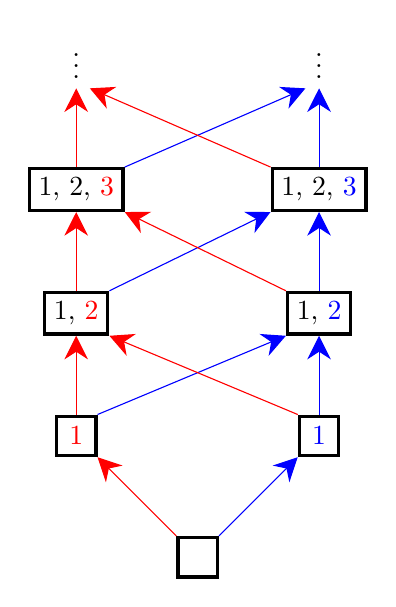
\begin{tikzpicture}[squarednode/.style={rectangle, draw, very thick, minimum size=5mm}]
			\node[squarednode]      (0)   [] {$ $};
			\node[squarednode]      (1r)   [above right=of 0] {{\color{blue}$1$}};
			\node[squarednode]      (1l)   [above left=of 0] {{\color{red}$1$}};
			\node[squarednode]      (2r)   [above=of 1r] {{1, \color{blue}$2$}};
			\node[squarednode]      (2l)   [above=of 1l] {{1, \color{red}$2$}};
			\node[squarednode]      (3r)   [above=of 2r] {{1, 2, \color{blue}$3$}};
			\node[squarednode]      (3l)   [above=of 2l] {{1, 2, \color{red}$3$}};
			\node      (4r)   [above=of 3r] {{$\vdots$}};
			\node      (4l)   [above=of 3l] {{$\vdots$}};
			\draw[-{Stealth[length=3mm, width=3mm]}, color=blue] (0.north east) -- (1r.south west);
			\draw[-{Stealth[length=3mm, width=3mm]}, color=red] (0.north west) -- (1l.south east);
			\draw[-{Stealth[length=3mm, width=3mm]}, color=blue] (1r.north) -- (2r.south);
			\draw[-{Stealth[length=3mm, width=3mm]}, color=red] (1l.north) -- (2l.south);
			\draw[-{Stealth[length=3mm, width=3mm]}, color=blue] (1l.north east) -- (2r.south west);
			\draw[-{Stealth[length=3mm, width=3mm]}, color=red] (1r.north west) -- (2l.south east);
			\draw[-{Stealth[length=3mm, width=3mm]}, color=blue] (2r.north) -- (3r.south);
			\draw[-{Stealth[length=3mm, width=3mm]}, color=red] (2l.north) -- (3l.south);
			\draw[-{Stealth[length=3mm, width=3mm]}, color=blue] (2l.north east) -- (3r.south west);
			\draw[-{Stealth[length=3mm, width=3mm]}, color=red] (2r.north west) -- (3l.south east);
			\draw[-{Stealth[length=3mm, width=3mm]}, color=blue] (3r.north) -- (4r.south);
			\draw[-{Stealth[length=3mm, width=3mm]}, color=red] (3l.north) -- (4l.south);
			\draw[-{Stealth[length=3mm, width=3mm]}, color=blue] (3l.north east) -- (4r.south west);
			\draw[-{Stealth[length=3mm, width=3mm]}, color=red] (3r.north west) -- (4l.south east);
		\end{tikzpicture}
	\end{center}
	\caption{Counter-model to $\varphi$.}
	\label{fig1}
\end{wrapfigure}

\begin{example}
	Consider $\varphi = \neg(\neg \forall xA(x)\vee\neg \forall xB(x))$. There is a counter-model as shown in Figure~\ref{fig1}
	where at each node the elements that exist at it are indicated. For black ones both $A$ and $B$ hold, for red ones only $B$, for blue ones only $A$. Furthermore red arrows indicate $f_{\neg \forall xA(x)}$ and blue arrows $f_{\neg \forall xB(x)}$. Note that applying $f_{\neg \forall xA(x)}$ we must always reach the left column and $f_{\neg \forall xB(x)}$ we must always reach the right column. Therefore applying $f_{\neg \forall xA(x)}\circ f_{\neg \forall xB(x)}$ we can never remain stationary. This is in contrast to the propositional case.
\end{example}

However Lemma~\ref{thm:fo-countermodel-reduction} still enables us to add some additional axioms which could help guide proof search. In particular we may assume that $f_\psi(w) = w$ if $\exists u(w = f_\psi(u))$ for $\psi\in\mathcal F_\forall$, i.e. $f_\psi$ is idempotent, and  $f_\psi(w) = w$ if $\exists u(w \geq f_\psi(u))$ for each $\psi\in\mathcal F_\to$, which is even stronger than idempotence. How adding these properties as assumption helps with proof search has to be examined.

\section{Conclusion}

We have presented embeddings of intuitionistic into classical logic for the propositional and the predicate case.
The transformation saw an exponential blow-up parameterized by $|\mathcal F_\to|$ in the propositional case and a complexity increase reflected by an arity-increase of one for all relations and the introduction of new function symbols in the predicate case.
A key motivation for our work is the potential of leveraging classical provers for showing intuitionistic validity.
%The practical feasibility of our translation is yet to be tested.
%In particular in the first-order case it is difficult to estimate how the increased complexity of the output formula impacts proof search.
Initial tests show promise but we plan on conducting a more thorough evaluation.
A key factor yet to be determined is how large the parameters $|\mathcal F_\to|$ in the propositional case and $|\mathcal F|$ in the predicate case are in practice.

The above mentioned complexity considerations are direct consequences of our straightforward constructions.
We plan to establish better bounds in future work by utilizing structural properties of the input formula, in particular by constructing smaller counter-examples $\mathcal M_T$ in case certain atoms are independent from each other.
On the theoretical side, we also hope to give a new translation from QBF to IPC that improves our understanding of the relationship between intuitionistic propositional logic and the polynomial hierarchy.

As a next step we will benchmark our translation using state-of-the art automated theorem provers, in particular the Vampire theorem prover~\cite{kovacs2013first}. We will have to adapt the counter-model translation to a proof translation for the particular calculus, e.g. superposition in the case of Vampire. Ultimately we hope that this will also open a new path for program extraction via the Curry-Howard Correspondence.


\bibliography{lipics-v2021-EIICL}

\appendix

\section{Omitted content}

\begin{lemma}\label{ap1}
	Let $\chi$ be a formula and $\{z_1\dots z_n\} = Z$ contain all free variables in $\chi$, then for every structure $\mathcal M = (M, I)$ there exists $\mathcal M_\chi = (M, I_\chi$) such that $p^{I_{\chi}} = p^I$ for all function and relation symbols $p$ occurring in $\chi$ and for all variable assignments $v$ we have
	\begin{itemize}
		\item if $\models\chi$ then $\mathcal M_\chi, v\models\chi^S_T$.
		\item if $\mathcal M, v\not\models\chi$ then $\mathcal M_\chi, v\not\models\chi^H_T$.
	\end{itemize}
\end{lemma}

\begin{proof}
	We proceed by simultaneous induction on the formula height.
	
	For atomic $\chi$ the claims are clear.
	
	Otherwise there are $3$ cases:
	
	1. $\chi = \varphi\circ\psi$ for $\circ\in\{\wedge,\vee,\to\}$. By induction hypothesis there exist $\mathcal M_{\varphi, v} = (M, I_{\varphi, v}), \mathcal M_{\psi, v} = (M, I_{\psi, v})$ for $\varphi,\psi$ as in the lemma. Then we can define $I_{\chi, v}$ as follows:
	
	For every symbol $p$ that occurs in $\varphi^S$ or $\varphi^H$ but not $\psi^S, \psi^H$ have $p^{I_{\chi, v}} = p^{I_{\varphi, v}}$. For every symbol $p$ that occurs in $\psi^S$ or $\psi^H$ but not $\varphi^S, \varphi^H$ have $p^{I_{\chi, v}} = p^{I_{\psi, v}}$. Otherwise $p$ already occurs in $\varphi$ so have $p^{I_{\chi, v}} = p^I$.
	
	Let $\circ=\to$. Suppose $\mathcal M, v\models\chi$. Then $\mathcal M, v\not\models\varphi$ or $\mathcal M\models\psi$ and therefore $\mathcal M_\chi\not\models\varphi^S_T$ or $\mathcal M_\chi\models\psi^H_T$, i.e. $\mathcal M_\chi\models\chi^S_T$. On the other hand suppose $\mathcal M, v\not\models\chi$. Then $\mathcal M, v\models\varphi$ and $\mathcal M, v\not\models\psi$ and therefore $\mathcal M_\chi, v\models \varphi^S_T$ and $\mathcal M_\chi, v\not\models\psi^S_T$, i.e. $\mathcal M_\chi\not\models\chi^H_T$. Analogous arguments work for $\circ\in\{\wedge, \vee\}$.
	
	2. $\chi = \forall x\varphi$. Choose $s^{I_\chi}:M^n\to M$ such that $s^{I_\chi}(x_1,\dots, x_n) = m$ if there exists $m\in M$ such that $\mathcal M, v[x_1/t_1\dots x_n/t_n, m/a]\not\models\varphi[a/x]$ for all $v$ and arbitrary otherwise. Since $T$ contains all free variables occurring in $\chi$ this is a well-defined function.
	
	By induction hypothesis there exists a structure $\mathcal M_{\varphi[a/x]}$ as is the Lemma. Let $p^{I_\chi} = p^{I_{\varphi[a/x]}}$ for all symbols occurring in $\chi$ and $$p^{I_\chi}(x_1\dots x_{i-1}, x_{i+1}\dots x_m) = p^{I_{\varphi[a/x]}}(x_1\dots x_{i-1}, s^{I_\chi}(x_1\dots x_n), x_{i+1}\dots x_m)$$ for all symbols $p$ occurring in $\varphi[a/x]^S_{T\cup a}$ or $\varphi[a/x]^H_{T\cup a}$ but not in $\chi$ where $x_i$ is the argument corresponding to the free variable $a$.
	
	Suppose $\mathcal M, v\models\chi$. Then for all $m\in M$ $\mathcal M, v[m/a]\models\varphi[a/x]$ and therefore $\mathcal M_{\chi}, v[m/a]\models\varphi[a/x]^S_{M\cup\{a\}}$ and thus $\mathcal M_{\chi}, v\models \forall x\varphi([a/x]^S_{M\cup\{a\}}[x/a])$, i.e. $\mathcal M_\chi,v\models \chi^S$. On the other hand suppose $\mathcal M, v\not\models\chi$. Then there exists $m\in M$ such that $\mathcal M, v[m/a]\not\models\varphi[a/x]$ and therefore $\mathcal M_\chi, v[m/a]\not\models\varphi[a/x]^H_{T\cup\{a\}}$ and so by definition $\mathcal M_\chi, v\not\models\varphi[s(t_1,\dots t_n)/x]^H_T$, i.e. $\mathcal M_\chi, v\not\models(\forall x\varphi)^H_T$.
	
	3. $\chi = \exists x\varphi$. The argument runs dually to 2. Choose $s^{I_\chi}:M^n\to M$ such that $s^{I_\chi}(x_1,\dots, x_n) = m$ if there exists $m\in M$ such that for all $v$ we have $\mathcal M, v[x_1/t_1\dots x_n/t_n, m/a]\models\varphi[a/x]$ and arbitrary otherwise. Since $T$ contains all free variables occurring in $\chi$ this is a well-defined function.
	
	By induction hypothesis there exists a structure $\mathcal M_{\varphi[a/x]}$ as is the Lemma. Let $p^{I_\chi} = p^{I_{\varphi[a/x]}}$ for all symbols occurring in $\chi$ and $$p^{I_\chi}(x_1\dots x_{i-1}, x_{i+1}\dots x_m) = p^{I_{\varphi[a/x]}}(x_1\dots x_{i-1}, s^{I_\chi}(x_1\dots x_n), x_{i+1}\dots x_m)$$ for all symbols $p$ occurring in $\varphi[a/x]^S_{T\cup a}$ or $\varphi[a/x]^H_{T\cup a}$ but not in $\chi$ where $x_i$ is the argument corresponding to the free variable $a$.
	
	Then as in 2 from $\mathcal M, v\models \chi$ follows $\mathcal M_\chi,v\models\chi^S_T$ and from $\mathcal M, v\not\models \chi$ follows $\mathcal M_\chi,v\not\models\chi^H_T$.
\end{proof}

\begin{lemma}\label{ap2}
	For every structure $\mathcal M$ and $\{t_1\dots t_n\} = T$ that contains all free variables in $\chi$ and variable assignment $v$
	\begin{itemize}
		\item if $\mathcal M, v\models\varphi^S_T$ then $\mathcal M, v\models \varphi$
		\item if $\mathcal M, v\not\models\varphi^H_T$ then $\mathcal M, v\not\models\varphi$.
	\end{itemize}
\end{lemma}

\begin{proof}
	Again we proceed by simultaneous induction on the formula height.
	
	For atoms the claims are clear. We distinguish 5 cases.
	
	1. $\chi = \varphi\to\psi$. Suppose $\mathcal M, v\models\chi^S_T$, i.e. $\mathcal M, v\not\models\varphi^H_T$ or $\mathcal M, v\models\psi^S_T$. By induction hypothesis $\mathcal M, v\not\models \varphi$ or $\mathcal M, v\models\psi$, i.e. $\mathcal M, v\models \chi$. On the other hand suppose $\mathcal M, v\not\models\chi^H_T$, i.e. $\mathcal M, v\models\varphi^S_T$ and $\mathcal M, v\not\models\varphi^H_T$. Again by induction hypothesis $\mathcal M,v\models\varphi$ and $\mathcal M, v\not\models \varphi$, so $\mathcal M, v\not\models\chi$.
	
	2. + 3. Conjunctions and Disjunctions are dealt with analogously.
	
	4. $\chi = \forall x\varphi$.  Suppose $\mathcal M, v\models\chi^S_T$, i.e. for all $m\in M$ we have $\mathcal M, v[m/a]\models \chi[a/x]^S_{T\cup\{a\}}$ and by induction hypothesis $\mathcal M, v[m/a]\models \chi[a/x]$. Then it follows that $\mathcal M, v\models\varphi$. On the other hand suppose $\mathcal M, v\not\models\chi^H_T$, i.e. there exists $m\in M$ such that $\mathcal M, v[m/a]\not\models\chi[a/x]^H_{T\cup \{a\}}$, then by induction hypothesis $\mathcal M, v[m/a]\not\models \chi[a/x]$, i.e. $\mathcal M, v\not\models\forall x\chi$.
	
	5. $\chi = \exists x\varphi$.  The argument runs dually to 4.
\end{proof}

\begin{definition}\label{def:transf-structure}
	For every classical and intuitionistic structure $\mathcal M$ define a structure $\mathcal S(\mathcal M,\varphi)$ that agrees with $\mathcal M$ on everything except the interpretation(s) of atoms of the form $P_\psi$. By slight abuse of notation we denote with $\vec z_\psi$ elements of the domain instead of variables. In the classical case have
	$$\begin{matrix}
		P_A^I(\vec z_A):\Leftrightarrow A^I(\vec z_A)\\
		P_{\varphi\wedge\psi}^I(\vec z_{\varphi\wedge\psi}) :\Leftrightarrow P_{\varphi}^I(\vec z_\varphi)\wedge P_{\psi}^I(\vec z_\psi)\indent P_{\varphi\vee\psi}^I(\vec z_{\varphi\vee\psi}) :\Leftrightarrow P_{\varphi}^I(\vec z_\varphi)\vee P_{\psi}^I((\vec z_\psi))\\P_{\varphi\to\psi}^I(\vec z_{\varphi\to\psi}) :\Leftrightarrow (\neg P_{\varphi}^I(\vec z_{\varphi}))\vee P_{\psi}^I(\vec z_{\psi})\\P_{\forall x\varphi}^I(\vec z_{\forall x\varphi}) :\Leftrightarrow \{\vec z\:|\:\:P_{\varphi}^I(\vec z_\varphi) \text{ for all $x\in M$}\}\indent P_{\exists x\varphi}^I(\vec z_{\exists x\varphi}) :\Leftrightarrow \{\vec z\:|\:\:P_{\varphi}^I(\vec z_\varphi) \text{ for some $x\in M$}\}
	\end{matrix}$$
	and for intuitionistic logic and each world $u$
	$$\begin{matrix}
		P_A^{I_u}(\vec z_A):\Leftrightarrow A^{I_u}(\vec z_A)\\
		P_{\varphi\wedge\psi}^{I_u}(\vec z_{\varphi\wedge\psi}) :\Leftrightarrow P_{\varphi}^{I_u}(\vec z_\varphi)\wedge P_{\psi}^{I_u}(\vec z_\psi)\indent P_{\varphi\vee\psi}^{I_u}(\vec z_{\varphi\vee\psi}) :\Leftrightarrow P_{\varphi}^{I_u}(\vec z_\varphi)\vee P_{\psi}^{I_u}((\vec z_\psi))\\
		P_{\varphi\to\psi}^{I_u}(\vec z_{\varphi\to\psi}) :\Leftrightarrow(\neg P_{\varphi}^{I_w}(\vec z_{\varphi}))\vee P_{\psi}^{I_w}(\vec z_{\psi})\text{ for all $w\geq u$}\\
		P_{\forall x\varphi}^{I_u}(\vec z_{\forall x\varphi}) :\Leftrightarrow P_{\varphi}^{I_w}(\vec z_\varphi) \text{ for all $w\geq u$, $x\in M_w$}\indent P_{\exists x\varphi}^{I_u}(\vec z_{\exists x\varphi}) :\Leftrightarrow P_{\varphi}^{I_u}(\vec z_\varphi) \text{ for some $x\in M_u$}
	\end{matrix}$$
\end{definition}

\begin{lemma}~\label{thm:prop-countermodel-reduction2}
	Let $\mathcal M = (M, I)$ be a counter-model to $\mathcal \varphi^\circ$.
	\begin{enumerate}
		\item $\psi$ is fulfilled at $f_\psi^I(u)$ for all $u\in M, \psi\in\mathcal F_\to$.
		\item If $\psi$ is fulfilled at some $u\in M$ then $\psi$ is fulfilled at all $w\geq u$.
	\end{enumerate}
\end{lemma}

\begin{proof}
	1. If $C^I(u)$ is true then we are done due to persistency. Otherwise $C^I(u)$ is false.
	Because $(A^I(f_\psi^I(u))\to B^I(f_\psi^I(u)))\to C^I(u)$ holds, then $A^I(f_\psi^I(u))\to B^I(f_\psi^I(u))$ must be false.
	
	
	2. Let $w$ be some element with $w\geq u$.
	If $C^I(w)$ is true, we are done.
	Otherwise $C^I(w)$ is false.
	Due to persistency $C^I(u)$ is also false.
	Because $\psi$ is fulfilled at $u$, $A^I(u)\to B^I(u)$ must be false, i.e. $A^I(u)$ is true and $B^I(u)$ is false. Then $A^I(w)$ and $A^I(f^I_\psi(w))$ are also true due to persistency.
	Because $(A^I(f^I_\psi(w))\to B^I(f^I_\psi(w)))\to C^I(w)$ holds, we now get that  $B^I(f^I(w))$ must be false.
	But then due to persistency so is $B^I(w)$ and we have that $\psi$ is fulfilled at $w$.
\end{proof}

\begin{example}\label{ex:prop-tree-model}
	This is an example for the model translation from Corollary~\ref{cor:prop-tree-model}. Consider
	$$\mathcal S = \{(A\to B)\to C, (B\to A)\to D, (A\wedge B)\to \bot, (C\vee D)\to E\}$$and $\varphi = \bigwedge S\to E$ which has the Kripke counter-model, depicted below,
	\begin{center}
		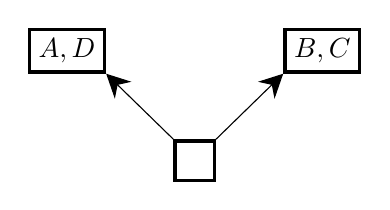
\begin{tikzpicture}[squarednode/.style={rectangle, draw, very thick, minimum size=5mm}]
			\node (center) {};
			\node[squarednode]      (right)   [right=of center] {$B, C$};
			\node[squarednode]      (left)    [left=of center] {$A, D$};
			\node[squarednode]      (lower)       	[below=of center] {};
			\draw[-{Stealth[length=3mm, width=3mm]}] (lower.north west) -- (left.south east);
			\draw[-{Stealth[length=3mm, width=3mm]}] (lower.north east) -- (right.south west);			
		\end{tikzpicture}
	\end{center}
	\vspace*{-.3cm}where at each node the true propositions are indicated.
	%	
	There is a corresponding classical counter-model $\mathcal M = (M, I)$ to $\varphi^\circ$ with $M = \{u, u_l, u_r\}$, $A^{I}(l) = D^I(l) = B^I(r) = C^I(r) = 1$ and $0$ else.
	%
	Denoting $\psi_1 := (A\to B)\to C$ and $\psi_2 := (A\to B)\to D$, this corresponds to a transformed counter-model $\mathcal M_T = (M_T, I_T)$ of $\varphi^\circ$ with $M_T = \{\epsilon, \psi_1, \psi_2, \psi_1\psi_2, \psi_2\psi_1\}$ and interpretation as presented below:
	\begin{center}
		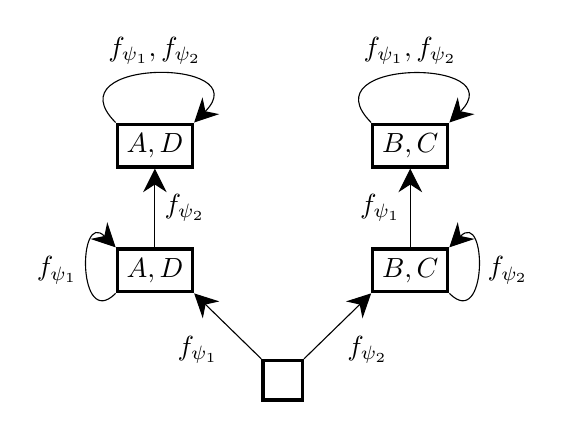
\begin{tikzpicture}[squarednode/.style={rectangle, draw, very thick, minimum size=5mm}]
			\node (center) {};
			\node[squarednode]      (right1)   [right=of center] {$B, C$};
			\node[squarednode]      (right2)   [above=of right1] {$B, C$};
			\node[squarednode]      (left1)    [left=of center] {$A, D$};
			\node[squarednode]      (left2)    [above=of left1] {$A, D$};
			\node[squarednode]      (lower)       	[below=of center] {};
			\draw[-{Stealth[length=3mm, width=3mm]}] (lower.north west) -- (left1.south east) node [midway, below left] {$f_{\psi_1}$};
			\draw[-{Stealth[length=3mm, width=3mm]}] (lower.north east) -- (right1.south west) node [midway, below right] {$f_{\psi_2}$};
			\draw[-{Stealth[length=3mm, width=3mm]}] (left1.north) -- (left2.south) node [midway, right] {$f_{\psi_2}$};
			\draw[-{Stealth[length=3mm, width=3mm]}] (right1.north) -- (right2.south) node [midway, left] {$f_{\psi_1}$};
			\draw[-{Stealth[length=3mm, width=3mm]}] (left1.south west) to [out=225, in=135, loop, looseness=3] node [left] {$f_{\psi_1}$} (left1.north west);		
			\draw[-{Stealth[length=3mm, width=3mm]}] (right1.south east) to [out=315, in=45, loop, looseness=3] node [right] {$f_{\psi_2}$} (right1.north east);
			\draw[-{Stealth[length=3mm, width=3mm]}] (left2.north west) to [out=135, in=45, loop, looseness=3] node [midway, above] {$f_{\psi_1}, f_{\psi_2}$} (left2.north east);
			\draw[-{Stealth[length=3mm, width=3mm]}] (right2.north west) to [out=135, in=45, loop, looseness=3] node [midway, above] {$f_{\psi_1}, f_{\psi_2}$} (right2.north east);		
		\end{tikzpicture}
	\end{center}
\end{example}


\begin{lemma}\label{lemma:QBF}
	$\varphi$ is not intuitionistically valid iff $\varphi^Q$ is a satisfiable QBF.
\end{lemma}
\begin{proof}
	Suppose $\varphi$ is not intuitionistically valid i.e. it $\bigwedge\mathcal S\to P$ has an intuitionistic counter-model. Then by the precious section there exists a classical counter-model $\mathcal M$ for $\bigwedge\mathcal S^\#\to P^\epsilon$.
	For each atom $A$ interpret $A^0$ such as $\mathcal M$ interprets $A^\epsilon$. Suppose we are given interpretations of all atoms $A^i$ for $i < n$ and a sequence with no repetitions $\psi_1\dots\psi_{n-1}$ over $\mathcal F_\to$ such that $\psi_i$ is exactly the $\psi\in\mathcal F_\to$ for which $F_{\psi}^i$ is true and $A^i$ is interpreted as $A^{\psi_1\dots\psi_i}$ is in $\mathcal M$.
	
	Let the $F^{n}_\psi$ be arbitrarily interpreted (since they are $\forall$-quantified). If not exactly one is interpreted as true then valid$(n)$ fails, i.e. have $\psi_n\in\mathcal F_\to$ the only element with $F^n_{\psi_n} = 1$. If $F^i_{\psi_n} = 1$ for some $i < n$ then valid$(n)$ also fails, so we may assume that $\psi_1\dots\psi_n$ is a sequence with no repetitions. Interpret the atoms $A^n$ as $\mathcal M$ interprets $A^{\psi_1\dots\psi_n}$. Continue this construction until $n  = |\mathcal F_\to|$. Then from $\mathcal M$ being a counter-example to $\mathcal S^\#\to P$ it directly follows that this interpretation satisfies $\varphi^Q$.
	
	On the other hand suppose $\varphi^Q$ is satisfiable. We construct a counter-example to $\varphi^\#$.
	Again we proceed iteratively. Interpret $A^\epsilon$ such as $A^0$ is interpreted in some satisfying interpretation of $\varphi^Q$. Suppose we are given a sequence $\psi_1\dots \psi_{n-1}$ such that for $i<n$ having $A^i = A^{\psi_0\dots\psi_{n-1}}$ is part of a satisfying interpretation of $\varphi^Q$ in which $F^i_\psi$ is chosen true iff $\psi = \psi_i$. Let $\psi_n\in\mathcal F_\to$. Consider some interpretation of the $A^n$ that are part of a satisfying assignment where $F^n_\psi$ is true iff $\psi = \psi_n$ and all variables quantified above are chosen as before. Have $A^{\psi_0\dots\psi_n} = A^n$ for each propositional variable $A$. From the definitions it directly follows that construction yields a counter-model for $\varphi^\#$.
\end{proof}

\begin{lemma}\label{lemma:fo-simplification}
	$\varphi$ is intuitionistically valid if and only of $\varphi^\circ$ is classically valid.
\end{lemma}

\begin{proof}
	We proceed by translation of counter-examples. Suppose first we have a counter-example $\mathcal M = (M, I)$ to $\varphi^\circ$. As a Kripke frame $(W, \leq)$ take all $ W = \{m\in M\:|\:\text{ World}^I(m)\}$ let $\leq$ be $\preceq^I$ restricted to $W$. Then let $M_u = \{m\in M\:|\: E(m, u)\}$ and let $f^{I_u}$ be $f^I$ restricted to $M_u$ and $A^{I_u}(\vec x): \Leftrightarrow A^\#(\vec x, u)$. It is then a straightforward check of definitions that this defines a Kripke counter-model to $\varphi$.
	
	The other direction is a bit more involved. Suppose we have a Kripke counter-model to $\varphi$ with frame $(W, \preceq)$ and family of $\Sigma$-structures $(M_w, I_w)_{w\in W}$. In particular since it is a counter-model there exists $w_0\in W$ with $w_0\not\models\varphi$. Let $W_0 = \{w\in W\:|\: w\geq w_0\}$ and define an equivalence relation $\sim$ on $\{(x, u)\:|\:u\in W_0, x\in M_u\}$ via $(x, u)\sim (y, w)$ iff $x = y$ and there exists $v\in W_0$ comparable with both $u, w$ such that $x\in v$ and denote the equivalence class of $(x, u)$ with $[x, u]$. Let $M = W_0\cup \{[x, u]\:|\:u\in W_0, x\in M_u\}$.
	Now have
	\begin{itemize}
		\item $s^I = w_0$.
		\item $E^I(m, w)$ iff $w\in W_0$ and $m \sim [x, w]$ for some $x\in M_w$.
		\item $f^I(m_1\dots m_n) =\begin{cases}
			f^{I_u}(x_1\dots x_n), &\text{if there are $ u\in W_0, x_i\in M_u$ with $m_i\sim [x_i, u]$ for all $i$,}\\
			w_0, & \text{otherwise.}
		\end{cases}$
		\item ${A^\#}^I(m_1\dots m_n, u) \Leftrightarrow\begin{cases}
			A^{I_u}(x_1\dots x_n), &\text{if $u\in W_0$ and $\exists x_i\in M_u$ w. $m_i\sim [x_i, u]$ for all $i$,}\\
			\top, & \text{otherwise.}
		\end{cases}$
	\end{itemize}
	One easily verifies that these are well-defined. Let us now briefly check that this indeed defines a counter-model. First of all ${P^\#}^I(s^I)$ is false since $P^{I_{w_0}}$ is. Clearly World$(w_0)$ holds and $K(\varphi)$ is also easily verified. All that remains to show is $M, I\models\bigwedge\mathcal S^\circ$. Consider e.g. the case where $\psi\in\mathcal S$ is of the form
	$$ \forall \vec z((A(\vec a)\to B(\vec b))\to C(\vec c))$$
	We have to show that
	$$M, I\models \forall \vec z\forall u(\vec E(t, u)\to \forall w(u\preceq w\to A^\#(\vec a, w)\to B^\#(\vec b, w))\to C^\#(\vec c, u))$$
	holds. Suppose towards contradiction that it does not, i.e. there are $u, \vec z\in M$ such that for all $w\in M$
	$$\vec E^I(\vec z, u)\to (u\preceq w\to {A^\#}^I(\vec a, w)\to {B^\#}^I(\vec b, w))\to {C^\#}^I(\vec c, u)$$ is false. For that ${C^\#}^I(\vec c, u)$ must be false and in particular $u\in W_0$. Futhermore $\vec E^I(\vec z, u)$ must be true and we can write $\vec z = [z_1, u]\dots[z_n, u]$ for some $z_i\in W_u$. Note that the above is false in particular for $w\in M_0$ with $u\preceq w$. But this would imply
	$$((A^{I_u}(\vec a)\to B^{I_u}(\vec b))\to C^{I_u}(\vec c))[\vec z/z_1\dots z_n]$$in our original Kripke counter-model. The other cases are analogous.
\end{proof}


\end{document}
